\documentclass[12pt, a4paper]{article}
\usepackage[utf8]{inputenc}
\usepackage[margin=1.2in]{geometry}
\usepackage{listings}
\usepackage{setspace}
\usepackage{xcolor}
\usepackage{titlesec}
\usepackage{enumitem}
\usepackage{amssymb}
\usepackage{amsmath}
\usepackage{tocloft}
\usepackage{bm}
\usepackage{multicol}
\usepackage{graphicx}
\graphicspath{{./Figures/}}
\usepackage{color}
\usepackage{hyperref}
\hypersetup{
	colorlinks=true,
	linkcolor=blue,
	urlcolor=blue,
	linktoc=none
}
\titleformat*{\section}{\Large\bfseries}
\titleformat*{\subsection}{\large\bfseries}
\renewcommand\thesection{\Roman{section}.}
\renewcommand\thesubsection{\alph{subsection}.}
\addtolength{\cftsecnumwidth}{16pt}

\begin{document}
\begin{spacing}{1.1}

	\begin{titlepage}
		\begin{center}
			\vspace*{1.4cm}
			
			\Huge \textbf{Capstone Project Report}
			
			\vspace*{1cm}
			
			
\includegraphics[scale=.5]{logo}
			
			\vspace*{1cm}
			
			\LARGE {Udacity Machine Learning Engineer Nanodegree}
			
			\vspace*{1cm}
			
			\hrule \vspace*{.5cm}
			
			\Large \textbf{A capstone report for analyzing worldwide food production and population from 1961-2013.}
			
			\vspace*{.5cm} \hrule
			
			\vspace*{1cm}
			
			\Large Derek Helms \\
			\Large January 25$^{th}$, 2021
		\end{center}
	\end{titlepage} \newpage

	\begin{titlepage}
		\vspace*{3cm}
		\renewcommand*\contentsname{Table of Contents}
		\tableofcontents
	\end{titlepage} \newpage

%%%% PAGE 1 %%%%

	\section{Definition}
	\subsection{Project Overview}
	The current world population is nearly 7.8 billion people, and this number is estimated to rise to around 9.7 billion in the year 2050. This means within the next 30 years, we will need to feed two billion more people without sacrificing the planet (1). This means we will need to double our crop production in order to feed that growing population. Agriculture is one of the greatest contributors of global warming, with farming consuming immense amounts of our water supplies and leaving major pollutants as its byproduct from fertilizer runoff (4). \vspace*{2mm}\\	
	Two different datasets were used in the analysis, one coming from \href{https://www.kaggle.com/dorbicycle/world-foodfeed-production}{Kaggle} and one coming from \href{http://www.fao.org/faostat/en/#data/OA}{FAO} (the Food and Agriculture Organization of the United Nations).\vspace*{2mm}\\	
	The dataset obtained through Kaggle is a Food Balance Sheet that originated from FAO's database, but has been formatted for easy of use, with a total of 63 features and 21477 observations. Food Balance Sheets represent the pattern of a country's food supply during a period of time, in this case it is yearly from 1961 to 2013, and measured in 1000 tonnes (2)
	\begin{center}	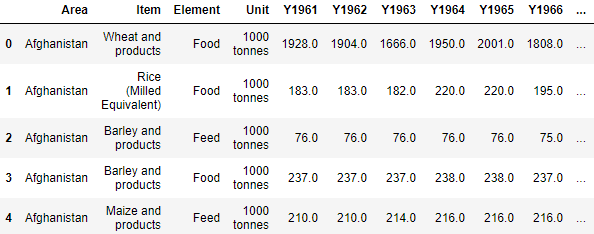
\includegraphics[scale=.9]{food_data}	\end{center}
	The dataset obtained through FAO is a time series dataset that contains the estimated/projected population (for both sexes) in each country from 1961 to 2018. The estimates are based on data from the World Population Prospects and World Urbanization Prospects (3).
	\begin{center}	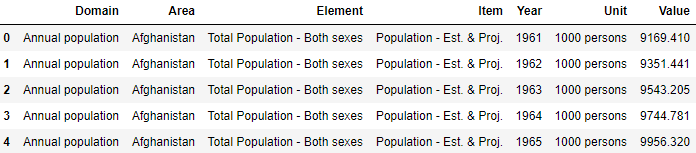
\includegraphics[scale=.8]{pop_data}	\end{center} \newpage

%%%% PAGE 2 %%%%

	\noindent The use cases for each dataset is as follows. The Kaggle dataset will be used in analyzing food production, seeing which countries produce the most and if it is for human or livestock consumption. This data will also be used to cluster countries together based on their production levels, ideally separating high and low producing countries. The FAO dataset will be used to compare the global population to the yearly total food production, as well as further analyzing the highest producing countries to see if they have the largest/fastest increasing populations.	
	
	\subsection{Problem Statement}
	With a continuously growing population this leads to the question, how do we supply the necessary amount of food for an increasing world population without sacrificing the climate of our planet? There are many solutions to this question, but the focus of this capstone will be on analyzing the global production of consumables, as well as the ratio of food (human consumption) to feed (livestock consumption) produced by each country. Only 55\% of the current world crop production is consumed by humans, with the remaining being fed to livestock. On top of this, nearly 25\% of the world's food calories are wasted before they can be consumed (4).\vspace*{2mm}\\	
	One aspect to explore is which food items are the most produced and the use case for those food items, whether they are for human or animal consumption. This will allow us to understand where a majority of our food is being directed, and as suggested by \href{https://www.nationalgeographic.com/foodfeatures/feeding-9-billion/}{National Geographic}, could a shift in diet lead to more crops being used for human consumption rather than livestock feed. Creating graphs to find insight will allow us to see how population change has correlated to food production, and what percentage of consumables are for humans compared to livestock. \vspace*{2mm}\\	
	The second aspect to explore is creating a linear model that can estimate the total global production needed for a given global population. This means correlating population and production in order to create a regression model that can predict the necessary production for the 2050 population. These will be compared to scientific articles that determine the necessary growth in production needed, and which model best fits these predictions.\vspace*{2mm}\\
	The last aspect of the data to explore is separating the countries into clusters based on their yearly production. Analyzing which countries are responsible for feeding the majority of the population, and how to ensure they can continue to do so. From this, we can also see which countries are not highly producing, and how we can aid them in increasing production if possible. \newpage

%%%% PAGE 3 %%%%

	\subsection{Metrics}
	To evaluate our graphing and data exploration, we can use the \href{http://www.fao.org/faostat/en/#rankings/countries_by_commodity}{FAO rankings} for countries by commodity, which we can then compare to our graphs to see if we have the data correctly labeled. This ranking allows us to see the top 20 country's that produce the most for each food item, as well as the top 20 food items produced by each country from the years 1961 to 2019.\vspace*{2mm}\\
	To evaluate our regression, we will use the root mean squared error (RMSE), in order to determine which line is best fitting our data. However, the 2050 estimate will also be used in determining the evaluation of the model in order to avoid overfitting the original data and having a poor future estimate (since we know the production needs to be anywhere for 50-100\% increased). \vspace*{2mm}\\
	With the data being unlabeled, it will be difficult to ensure that our clusters are properly partitioned. However, we can analyze both the clusters and graphs we create using two separate methods. One metric we can use to evaluate our model will be a \href{https://scikit-learn.org/stable/auto_examples/cluster/plot_kmeans_silhouette_analysis.html}{silhouette score}, which will measure on a scale from [-1,1] how close each point on one cluster is to points in the neighboring clusters. We will want to aim for a silhouette coefficient near +1 to indicate that our samples are far away from neighboring clusters (5). \vspace*{2mm}\\
	To evaluate our graphing and data exploration, we can use the \href{http://www.fao.org/faostat/en/#rankings/countries_by_commodity}{FAO rankings} for countries by commodity, which we can then compare to our graphs to see if we have the data correctly labeled. This ranking allows us to see the top 20 country's that produce the most for each food item, as well as the top 20 food items produced by each country from the years 1961 to 2019. \vspace*{2mm}
	
	\section{Analysis}
	This is where the majority of the project has taken place, in exploring the data and creating visualizations in order to determine where the food we are producing is going, as well as who is responsible for producing it. The analysis was broken down into two different sections: production and population exploration. In the production section, we analyzed the top producing countries, explored the top produced food items, and finally the use case for the food items (food vs feed). In the population section, we analyzed population vs production, the populations for the top producing countries, and the largest population changes over the last 53 years. A more in-depth description and visualization will be given in the following two subsections. \newpage

%%%% PAGE 4 %%%%
	
	\subsection{Production Exploration}
	\textbf{Top 10 Producing Countries:}\\
	To begin the exploration, we wanted to graph the top 10 producing countries for global production from 1961 to 2013. After this, we compared total production for a given number of top countries to the rest of the world to see how much global production each are responsible for.
	\begin{center}
	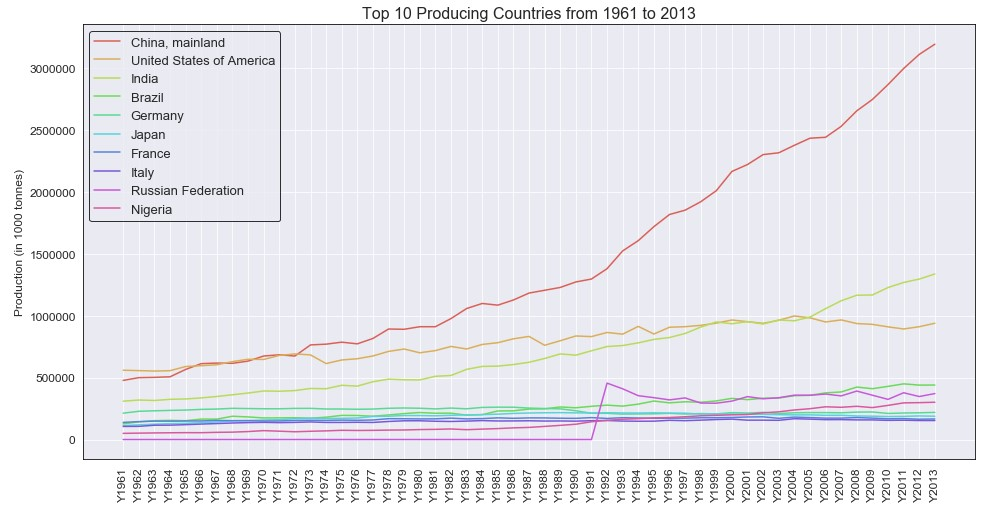
\includegraphics[scale=.58]{top_20_c_yearly} \vspace*{2mm}\\
	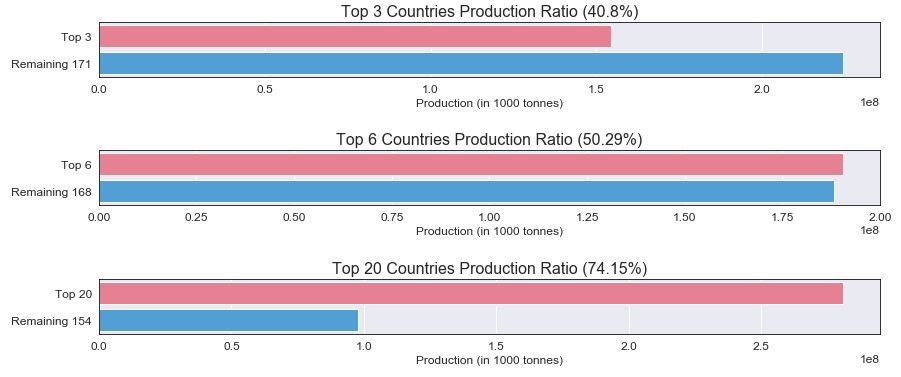
\includegraphics[scale=.58]{top_20_c_total}
	\end{center}
	From the line graph, we can see that the top 3 countries have been the top producers over the last 53 years. With China becoming dominant in the year 1972, it looks to be the beginning of an exponential growth pattern. The United States was second to China for a majority of the data, but seems to have plateaued and been passed by India starting in the early 2000's. India, being third highest of the data, has begun growing quickly since the late 1980's and seems to be increasing similar to China. An interesting finding is the Russian Federation spiking from 0 to nearly 500,000,000 tonnes of production from 1991 to 1992. \newpage

%%%% PAGE 5 %%%%
	
	\noindent This was due to the fact that the Russian Federation was found on December 25, 1991 and this was when our data begun with them (no production for Soviet Union was recorded in our data, which was the old name).\vspace*{2mm}\\
	Looking at the bar charts, and adding the three top producing countries together, it seems that they are responsible for around 40\% of the total global production. Going further, we can see that the top 6 producing countries are responsible for over 50\% of the global production, and the top 20 being responsible for 74\%. Out of 174 countries, it seems that only a small amount of them are responsible for the vast majority of production (however, these countries populations are also much larger than the others). \vspace*{6mm}\\
	\textbf{Exploring China's Production:}\\
	Being the top producer over the last 53 years (and most likely much before then), we want to further look into the production of the ``China, mainland" area. We will want to see what products make up a majority of their production, as well as the yearly breakdown to see any trends in production.
	\begin{center}
	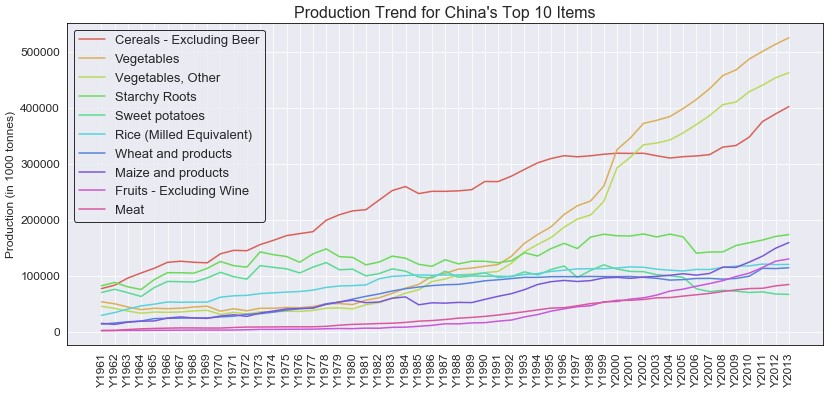
\includegraphics[scale=.65]{china_prod} 
	\end{center}
	From the graphs, we see that historically \textit{Cereals - Excluding Beer} has been the dominant product for China, but recently there has been a large spike in \textit{Vegetables} and \textit{Vegetables, Other} that has surpassed Cereals starting in the year 2000. However, Cereals seem to be rising again and could become the most produced item if Vegetables plateau. This is important to keep in mind for the next section of the exploration, where we looked at the top produced foot items. \newpage
	
%%%% PAGE 6 %%%%

	\noindent \textbf{Top Produced Items:}\\
	Initially, we wanted to separate the food and feed items from each other and create new datasets for both, in order to see how much is being produced for each use case. Although not all graphs can be included (a more in depth exploration and description can be seen in section 3.3 of the \textit{DataExploration} notebook), we will cover the main findings from the section.
	\begin{center}
	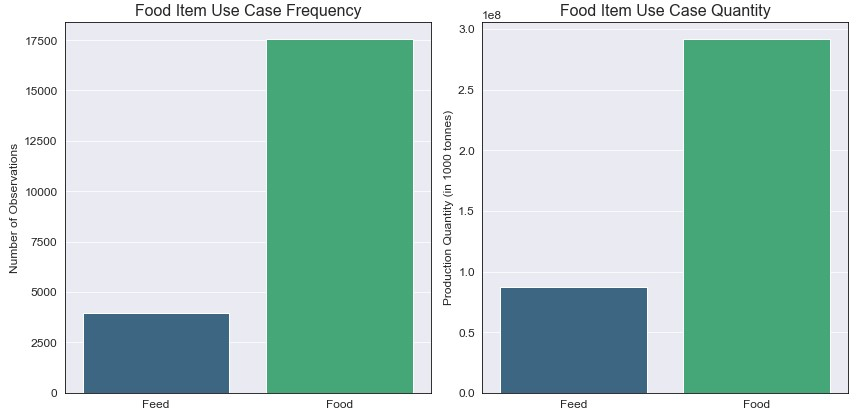
\includegraphics[scale=.65]{food_feed} 
	\end{center}
	We can see that a majority of the food is being used for human consumption, which is a good finding. There is around 3x more food (by weight) compared to feed, as well the dataset for food being around 4x larger than the feed dataset. 
	\begin{center}
	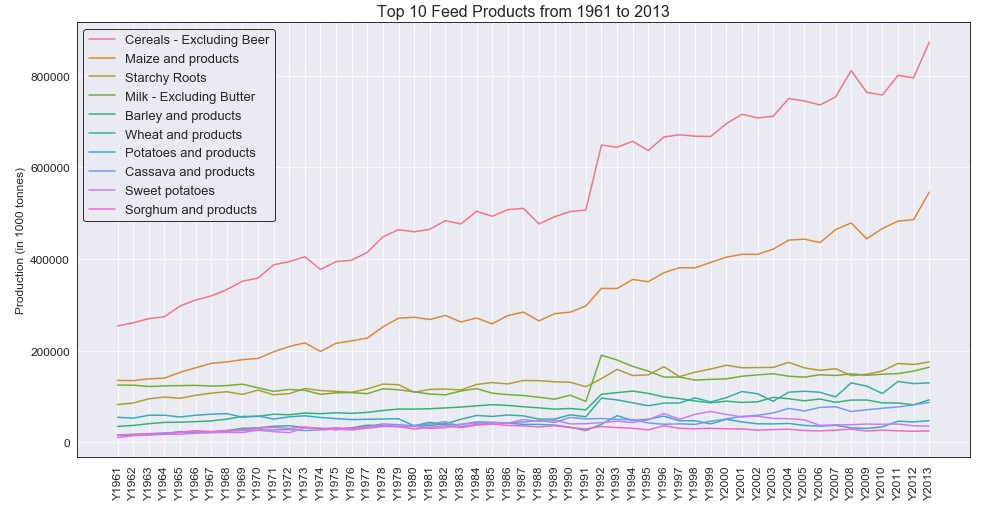
\includegraphics[scale=.6]{yearly_feed} 
	\end{center} \newpage

%%%% PAGE 7 %%%%

	\noindent For feed, the top product is "Cereals - Excluding Beer" by a landslide, with "Maize and products" coming in second (but at half the total production). Although no visual is included, there was an analysis to see which countries were the top producers for the top 2 items. It seems that the United States is clearly producing the most items for feed, with China being second to them. They produce the majority of the total, which is expected since they were both in the top 3 global producers.
	\begin{center}
	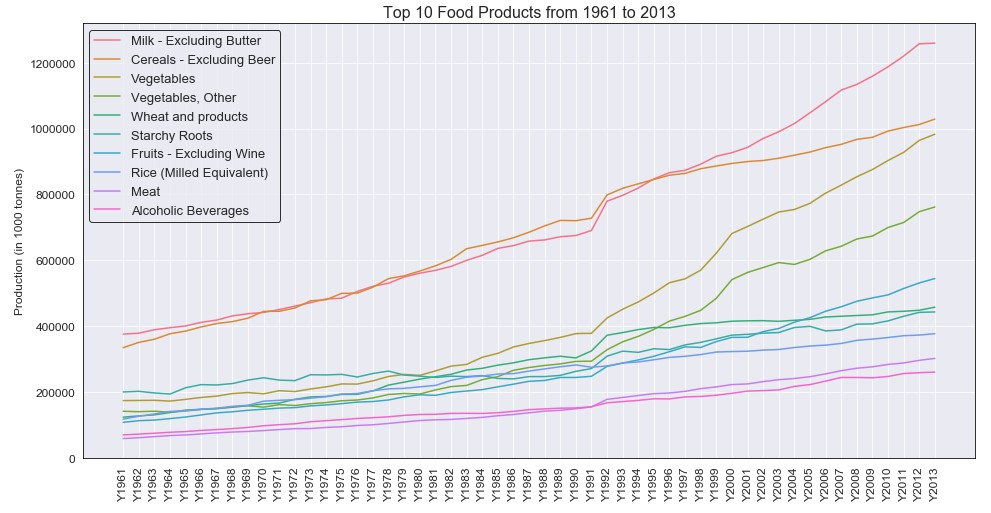
\includegraphics[scale=.6]{yearly_food} 
	\end{center}
	For food, there seemed to be a much closer grouping for production, which "Milk - Excluding Butter" and "Cereals - Excluding Beer" being the top 2 throughout most of the dataset, but "Vegetables" and "Vegetables - Other" seeming to be gaining traction and increasing quickly since the early 1990s. Again, an analysis was done to see who was the top producers for the food items, and it seems that China, India, and the United States were the main leaders for all of them (which is not surprising given our previous findings). \vspace*{2mm}
	
	\subsection{Population Exploration}
	Now that we understand the production, we also want to analyze the population for the countries. We will focus mainly on the top producing countries and their respective population, but before that we want to see any trends between population and production. \vspace*{2mm}\\
	To visualize these depictions, see section \textit{4.1: Population compared to Production} in the \textit{DataExploration} notebook. It seems that population is growing in a linear pattern, with population more than doubling in the last 53 years (1961-2013). \newpage
	
%%%% PAGE 8 %%%%

	\noindent Also, production and population seem the have a linear relationship (although not a completely straight line), which will be useful in the modeling section where we talk about the regression model we built. Now, we will look at the population compared to production for the top 3 countries (since they are responsible for over 40\% of the global production).
	\begin{center}
	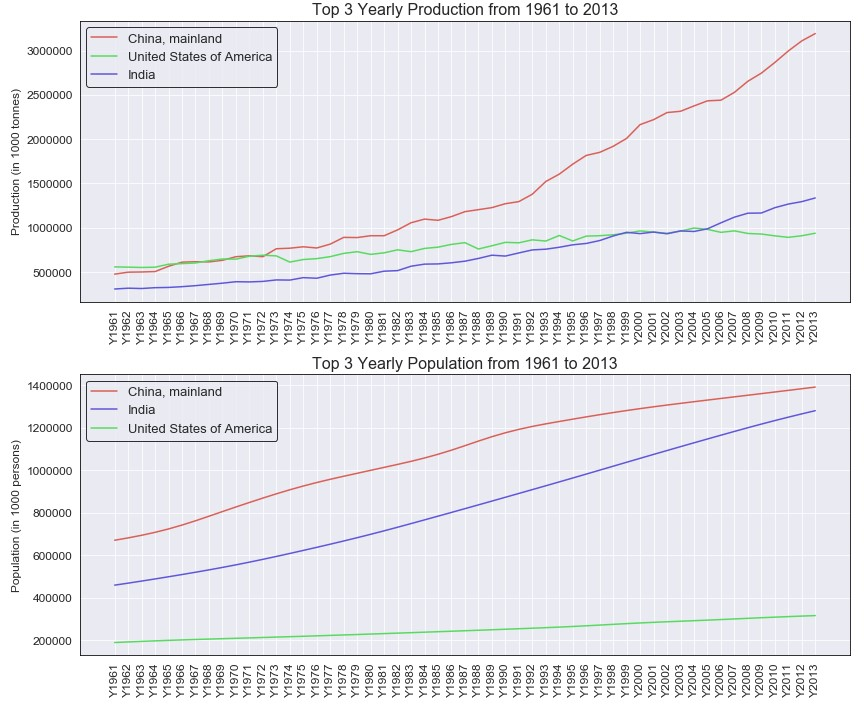
\includegraphics[scale=.63]{prod_pop} 
	\end{center}
	Looking at the production graph, the United States was the leader in yearly production, but they were quickly passed by China who began to grow rapidly in the 1970's. It also seems that since the early 1980's, India has been increasing and is following a similar pattern as China did in in the late 1960's. Looking at the population graph, we can see that over the past 53 years China has nearly doubled, India has grown almost 3x, and the United States has only grown around 1.5x. This could explain how India has passed the United States in production since the mid 2000's, with the US plateauing in production starting around 2000. \vspace*{2mm}\\
	Next, we wanted to see the yearly change for the most increased populations as well as the total population change over the last 53 years. A quick note: the yearly population is the increase from the previous year to the current year, so population is not dropping for negative slope but rather less people are being born or moving to certain countries. \newpage
	
%%%% PAGE 9 %%%%

	\begin{center}
	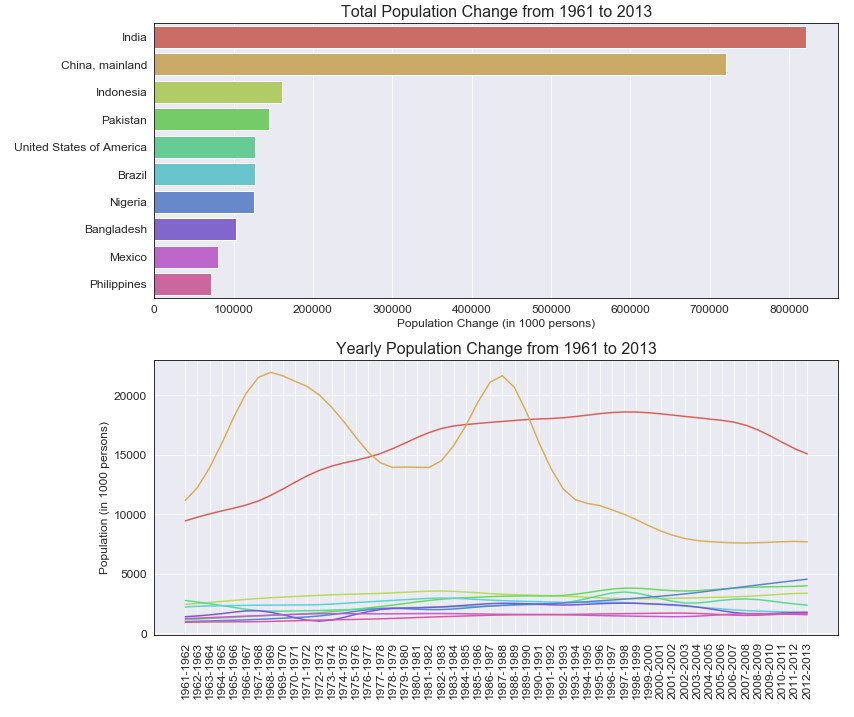
\includegraphics[scale=.65]{pop_change} 
	\end{center}
	Looking at our bar graph, we can see that again India and China have had the most people either born or immigrated into their countries by a landslide. The United States seems to be around 5th in terms of growth, with around less than 1/5 of the growth as China or India. We can see that India has had quite consistent growth, with a dropping increase in new people. China has fluctuated throughout the years, seeing large growth and small growth, but since the early 1990's it seems there is a decreasing number of new people each year. The remaining countries all have consistent growth, with around 1-5 million new people each year for the most part (including the United States). \vspace*{6mm}\\
	\textbf{Concluding Thoughts}:\\
	For this exploration, it is clear that China, India, and the United States are the top producing countries (but also the top populated countries). With around 40\% of the global production, it is crucial than we can continue to support these countries in order to ensure survival with an increasing need for food. We also saw that the majority of production is for humans and not livestock, which leads me to think that a shift in diet would not be necessary to supply more food globally. \newpage

%%%% PAGE 10 %%%%
	
	\section{Methodology}
	\subsection{Data Preprocessing}
	Two main things were done in the data preprocessing step: reformatting the population data to be similar to the production data layout (years as feature and Area as observations) and dropping China from the production dataset. \vspace*{2mm}\\
	Previously, the population data had each year being an observation for each country, but we wanted to have each year be a column and each country be an observation so that we could easily sum across the columns to get total yearly population. A function was written to do this for us (in the \textit{function.py} python module called \textit{format\_population\_data}) which followed the same layout as the production dataset and filled any missing years with \textit{NaN} values. Below is the original population format, followed by the new format:
	\begin{center}
	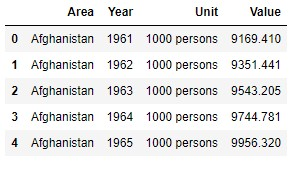
\includegraphics[scale=.7]{old_pop} \vspace*{2mm}\\
	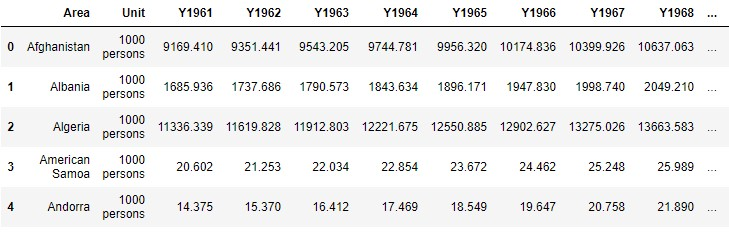
\includegraphics[scale=.7]{new_pop}
	\end{center}
	The next step we took was removing the general China area from the population dataset. This was because it was being double counted, since China was broken down into its regions (whose sum added up to the total China population). Also, the general area China is not in the production dataset (only its regions), so removing this was a key step in ensuring the population data was accurate. \vspace*{2mm}\\
	Note that removing China was built into the format population function, and the new formatted population dataset was outputted to the file ``FAO\_POP\_REFORMAT.csv". This was all done in the \textit{DataExploration} notebook in section 2. \newpage
	
%%%% PAGE 11 %%%%

	\subsection{Implementation}
	\textbf{Regression Models:}\\
	From our findings in the previous notebook, we noticed that yearly global population and yearly global production have a linear relationship. Using the estimated global population as the independent variable (y) and the global production as the dependent variable (x), we will estimate the total production that is expected given a total population value. This will allow us to see what the necessary production would be to support a given population. \vspace*{2mm}\\
	To begin, we want to create a base model using simple linear regression. This will allow us to see how the initial model performs, and how we can improve upon it.
	\begin{center}
	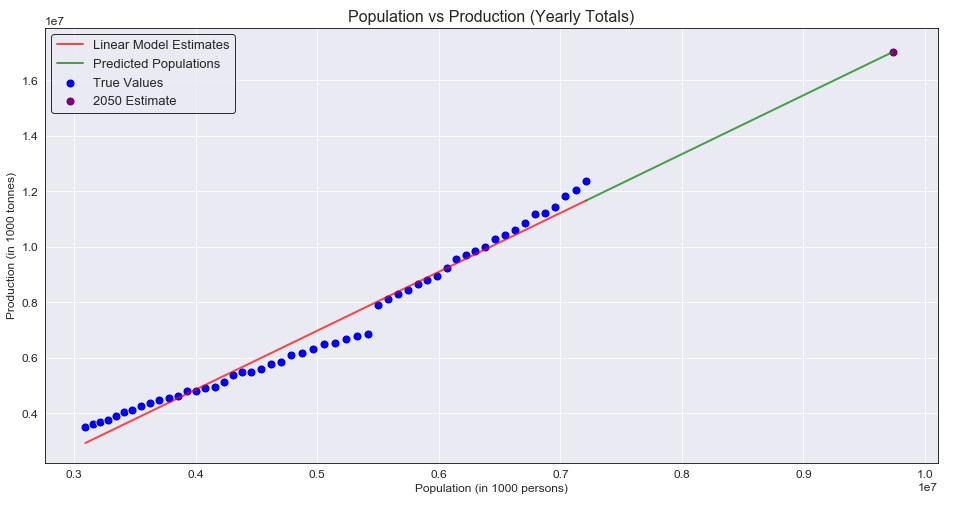
\includegraphics[scale=.6]{linear_model}
	\end{center}
	As we can see, the simple linear model does not fit our data very well, with an RMSE of around 405,000. However, its important to note that the data uses numbers in the millions, so the error was expected to be large. With an estimated production amount of 17013250 (in 1000 tonnes), this does not seem very accurate, since most experts say that we need to increase our production anywhere for 50-100\% to support to 2050 population. This was a good base model to indicate a base RMSE, but we will try to improve this model. A solution to this problem would be to fit a polynomial regression model that allows the line to bend and is better suited for the data. To do this, we will want to find out which degree minimizes the RMSE for the polynomial model, then use a subset of those to graph the predictions and see which model best represents our data. \vspace*{2mm}\\
	By graphing the RMSE and degree, we saw that a degree from 2-5 minimizes the RMSE, so we will want to create a polynomial model for each of these and compare. \newpage
	
%%%% PAGE 12 %%%%

	\begin{center}
	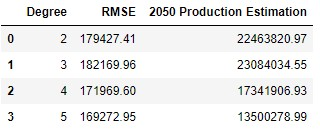
\includegraphics[scale=.85]{model_info} \\
	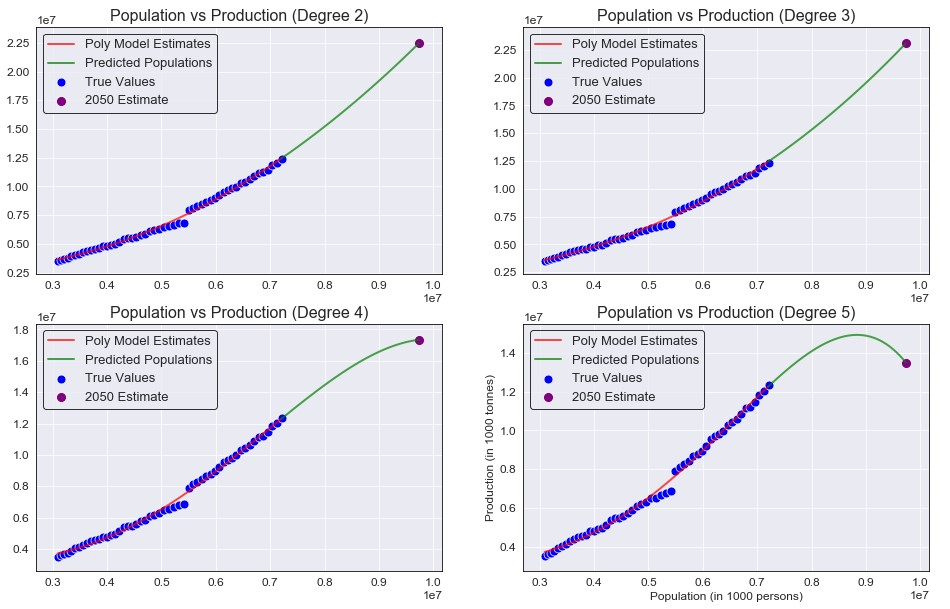
\includegraphics[scale=.61]{poly_model}
	\end{center}
	From the \href{https://www.wri.org/blog/2018/12/how-sustainably-feed-10-billion-people-2050-21-charts}{World Resources Institute}, we know that we need an increase of around 56\% in production from 2010 to 2050. The 2010 global production, from our dataset, was 11,445,072 (in 1000 tonnes). Following this idea, that means we need to produce 17,854,312.32 (in 1000 tonnes) total for the 2050 population. This seems to follow the degree 4 polynomial model, which estimated a production of 17,341,906.93 (in 1000 tonnes). \vspace*{2mm}\\
	However, from the \href{https://www.un.org/press/en/2009/gaef3242.doc.htm#:~:text=Food\%20production\%20must\%20double\%20by\%202050\%20to\%20meet\%20the\%20demand,a\%20panel\%20discussion\%20on\%20\%E2\%80\%9CNew}{United Nations}, we have also inferred that global food production must double in order to support the global population. Given that the article was written in 2009, with a global production of 11,211,891 (in 1000 tonnes) for out dataset, this means we need to produce 22,423,782 (in 1000 tonnes) for the year 2050. This idea follows the degree 2 model (almost exactly) with an estimated production of 22,463,820.97 (in 1000 tonnes).\vspace*{2mm}\\	
	Despite not being the lowest RMSE for the models, these 2 most accurately depict what has been estimated by professionals. Choosing which model is correct will be more of a challenge, since there is no real way to determine what the actual growth will be in the future (global events, pandemics, food supply, etc.). However, these two models are good indicators of a possible future that we could see. \newpage
	
%%%% PAGE 13 %%%% 

	\noindent \textbf{Clustering Model:}\\
	Next, we wanted to create a KMeans model to cluster countries together based on their production. We could have left the data how it was and use it for the clustering algorithm, but this resulted in extremely large inertia values (used below). To counter this, I used a z-score to standardize the data, which now is in the range [-0.322, 11.41], and our inertia is much more easily interpreted.
	\begin{center}
	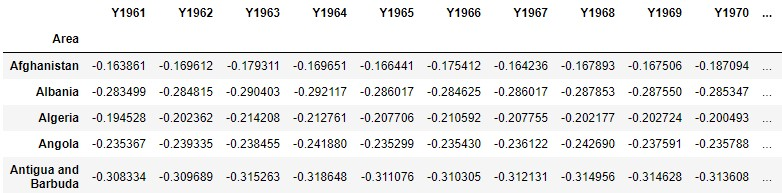
\includegraphics[scale=.7]{prod_z}
	\end{center}
	We needed a way to select the number of clusters, which we did by using the elbow method as well as silhouette scores. We want to choose $k$ where the inertia has the steepest slope, but the silhouette score that is closest to 1.
	\begin{center}
	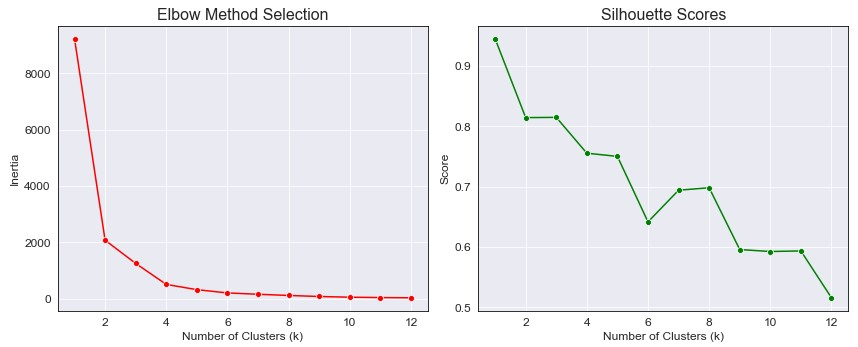
\includegraphics[scale=.7]{cluster_score}
	\end{center}
	Using the elbow method for the inertia graph, it seems that 2 is the ideal cluster number (but 3 and 4 could also be considered). We also used a silhouette score to determine help determine the number of clusters, which helps determine the distance between the resulting clusters, and we want a value of as close to 1 as possible. Using both of there, it seems that 2 clusters is ideal since this is where the elbow occurs and also has the highest silhouette score (besides 1 which is not considered in this case).\vspace*{2mm}\\	
	Finally, we created the model to group the countries together based on their production using 2 clusters. This was the initial guess we had, where we would separate the top 3 countries from the remaining since they had a much higher production compared to all the other countries. \newpage

%%%% PAGE 14 %%%%

	\begin{center}
	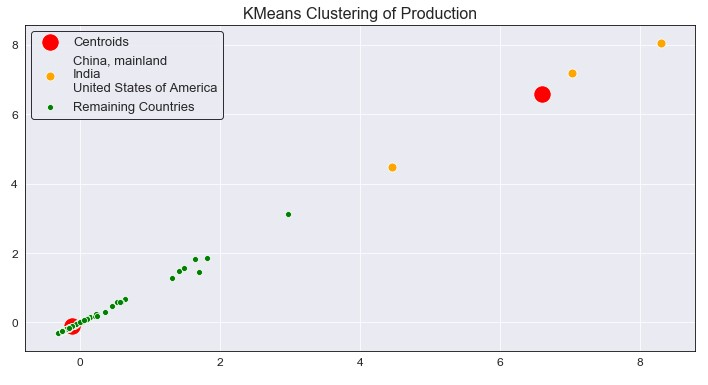
\includegraphics[scale=.8]{kmeans}
	\end{center}
	As expected, using 2 clusters separated the top 3 producers from the remaining countries. This means the clusters are based on high vs low production, since from the \textit{DataExploration} notebook we saw that the top 3 countries were responsible for over 40\% of the global production. The next closest country (Brazil) produced less than 1/3 the amount that the United States or India does and around 1/6 the amount of China. These clusters seem to be accurate in separating our data in correct clusters, and helps us visual how much more the top 3 countries produced compared to the remaining countries.\vspace*{2mm}
	
	\section{Results}
	

	





	\newpage
	
%%%% RESOURCES %%%%

	\section{Resources}
	$[1]$ Oppenheim, Dor. ``Who Eats the Food We Grow?" \textit{Kaggle}, 30 Nov. 2017, \\ \hspace*{5mm} www.kaggle.com/dorbicycle/world-foodfeed-production. \vspace*{2.5mm}\\
	$[2]$ ``Food Balances (Old Methodology and Population)." \textit{FAOSTAT}, Food and \\ \hspace*{5mm} Agriculture Organization of the United Nations, 12 Dec. 2017, \\ \hspace*{5mm} www.fao.org/faostat/en/\#data/FBSH. \vspace*{2.5mm}\\
	$[3]$ ``Annual Population." \textit{FAOSTAT}, Food and Agriculture Organization of the \\ \hspace*{5mm} United Nations, 16 Dec. 2019, www.fao.org/faostat/en/\#data/OA. \vspace*{2.5mm}\\
	$[4]$ Foley, Jonathan. ``A Five-Step Plan to Feed the World." \textit{Feeding 9 Billion - \\ \hspace*{5mm} National Geographic}, www.nationalgeographic.com/foodfeatures/feeding-9-billion/.\vspace*{2.5mm}\\
	$[5]$ ``Selecting the Number of Clusters with Silhouette Analysis on KMeans \\ \hspace*{5mm} Clustering." \textit{Scikit}, 
	\\ \hspace*{6mm} scikit-learn.org/stable/auto\_examples/cluster/plot\_kmeans\_silhouette\_analysis.html.\vspace*{2.5mm}\\
	$[6]$ Kiersz, Andy. ``The World Could Have Another Billion People in Thirteen \\\hspace*{6mm}Years." \textit{Business Insider}, Business Insider, 29 July 2015,\\\hspace*{6mm}www.businessinsider.com/un-world-population-projections-2015-7. \vspace*{2.5mm}\\
	


\end{spacing}
\end{document}